\documentclass[11pt, a4paper]{article}
\usepackage{pdfpages}
\usepackage{parallel}
\usepackage[T2A]{fontenc}
%\usepackage{ucs}
\usepackage[utf8]{inputenc}
\usepackage[english,russian]{babel}
\usepackage{hyperref}
\usepackage{rotating}
\usepackage[inner=2cm,top=1.8cm,outer=2cm,bottom=2.3cm,nohead]{geometry}
%\usepackage{listings}
\usepackage{graphicx}
\usepackage{wrapfig}
\usepackage{longtable}
\usepackage{indentfirst}
\usepackage{array}
\usepackage{tikzsymbols}
\usepackage{soul}
\usepackage[ruled,vlined]{algorithm2e}
\usepackage{qrcode}
\counterwithout{figure}{section} 

\usepackage{url}
\makeatletter
\g@addto@macro{\UrlBreaks}{\UrlOrds}
\makeatother

\newcolumntype{P}[1]{>{\raggedright\arraybackslash}p{#1}}
\frenchspacing
%\usepackage{fixltx2e} %text sub- and superscripts
\usepackage{icomma} % коскі ў матэматычным рэжыме
%\PreloadUnicodePage{4}

\newcommand{\longpage}{\enlargethispage{\baselineskip}}
\newcommand{\shortpage}{\enlargethispage{-\baselineskip}}

\def\switchlang#1{\expandafter\csname switchlang#1\endcsname}
\def\switchlangbe{
\let\saverefname=\refname%
\def\refname{Літаратура}%
\def\figurename{Іл.}%
}
\def\switchlangru{
\let\saverefname=\refname%
\let\savefigurename=\figurename%
\def\refname{Литература}%
\def\figurename{Рис.}%
}
\def\switchlangen{
\let\saverefname=\refname%
\def\refname{References}%
\def\figurename{Fig.}%
}

\hyphenation{admi-ni-stra-tive}
\hyphenation{ex-pe-ri-ence}
\hyphenation{fle-xi-bi-li-ty}
\hyphenation{Py-thon}
\hyphenation{ma-the-ma-ti-cal}
\hyphenation{re-ported}
\hyphenation{imp-le-menta-tions}
\hyphenation{pro-vides}
\hyphenation{en-gi-neering}
\hyphenation{com-pa-ti-bi-li-ty}
\hyphenation{im-pos-sible}
\hyphenation{desk-top}
\hyphenation{elec-tro-nic}
\hyphenation{com-pa-ny}
\hyphenation{de-ve-lop-ment}
\hyphenation{de-ve-loping}
\hyphenation{de-ve-lop}
\hyphenation{da-ta-ba-se}
\hyphenation{plat-forms}
\hyphenation{or-ga-ni-za-tion}
\hyphenation{pro-gramming}
\hyphenation{in-stru-ments}
\hyphenation{Li-nux}
\hyphenation{sour-ce}
\hyphenation{en-vi-ron-ment}
\hyphenation{Te-le-pathy}
\hyphenation{Li-nux-ov-ka}
\hyphenation{Open-BSD}
\hyphenation{Free-BSD}
\hyphenation{men-ti-on-ed}
\hyphenation{app-li-ca-tion}

\def\progref!#1!{\texttt{#1}}
\renewcommand{\arraystretch}{2} %Іначай формулы ў матрыцы зліпаюцца з лініямі
\usepackage{array}

\def\interview #1 (#2), #3, #4, #5\par{

\section[#1, #3, #4]{#1 -- #3, #4}
\def\qname{LVEE}
\def\aname{#1}
\def\q ##1\par{{\noindent \bf \qname: ##1 }\par}
\def\a{{\noindent \bf \aname: } \def\qname{L}\def\aname{#2}}
}

\def\interview* #1 (#2), #3, #4, #5\par{

\section*{#1\\{\small\rm #3, #4. #5}}
\ifx\ParallelWhichBox\undefined%
    \addcontentsline{toc}{section}{#1, #3, #4}%
\else%
\ifnum\ParallelWhichBox=0%
    \addcontentsline{toc}{section}{#1, #3, #4}%
\fi\fi%

\def\qname{LVEE}
\def\aname{#1}
\def\q ##1\par{{\noindent \bf \qname: ##1 }\par}
\def\a{{\noindent \bf \aname: } \def\qname{L}\def\aname{#2}}
}

\newcommand{\interviewfooter}[1]{
\vskip 1em
\noindent \textit{#1}
}

\AtEndDocument{\vfill\centering \qrcode{https://github.com/fiowro/mouses/blob/main/\jobname.pdf}}

\switchlang{en}
\begin{document}

\title{1984 -- Tektronix 4952 joystick}
\date{}
\author{~}
\maketitle
\selectlanguage{english}

Tektronix 4952 Joystick (fig. \ref{fig:TektronixJoystickPic}) was designed for the the 4010 series text-and-graphics computer terminals and similar 4050 series desktop computers based on storage-tube technology created by Tektronix to avoid the need for video RAM and still have high display resolutions of up to 1024x780 \cite{wiki}. Such devices were produced by Tektronix in the late 1970s through the early 1980s, until appearance of cheaper UNIX workstations. Adding joystick to the line of compatible peripheral devices was announced in 1974 \cite{adv}, while all known user manuals are dated with the next year or later.

\begin{figure}[h]
   \centering
    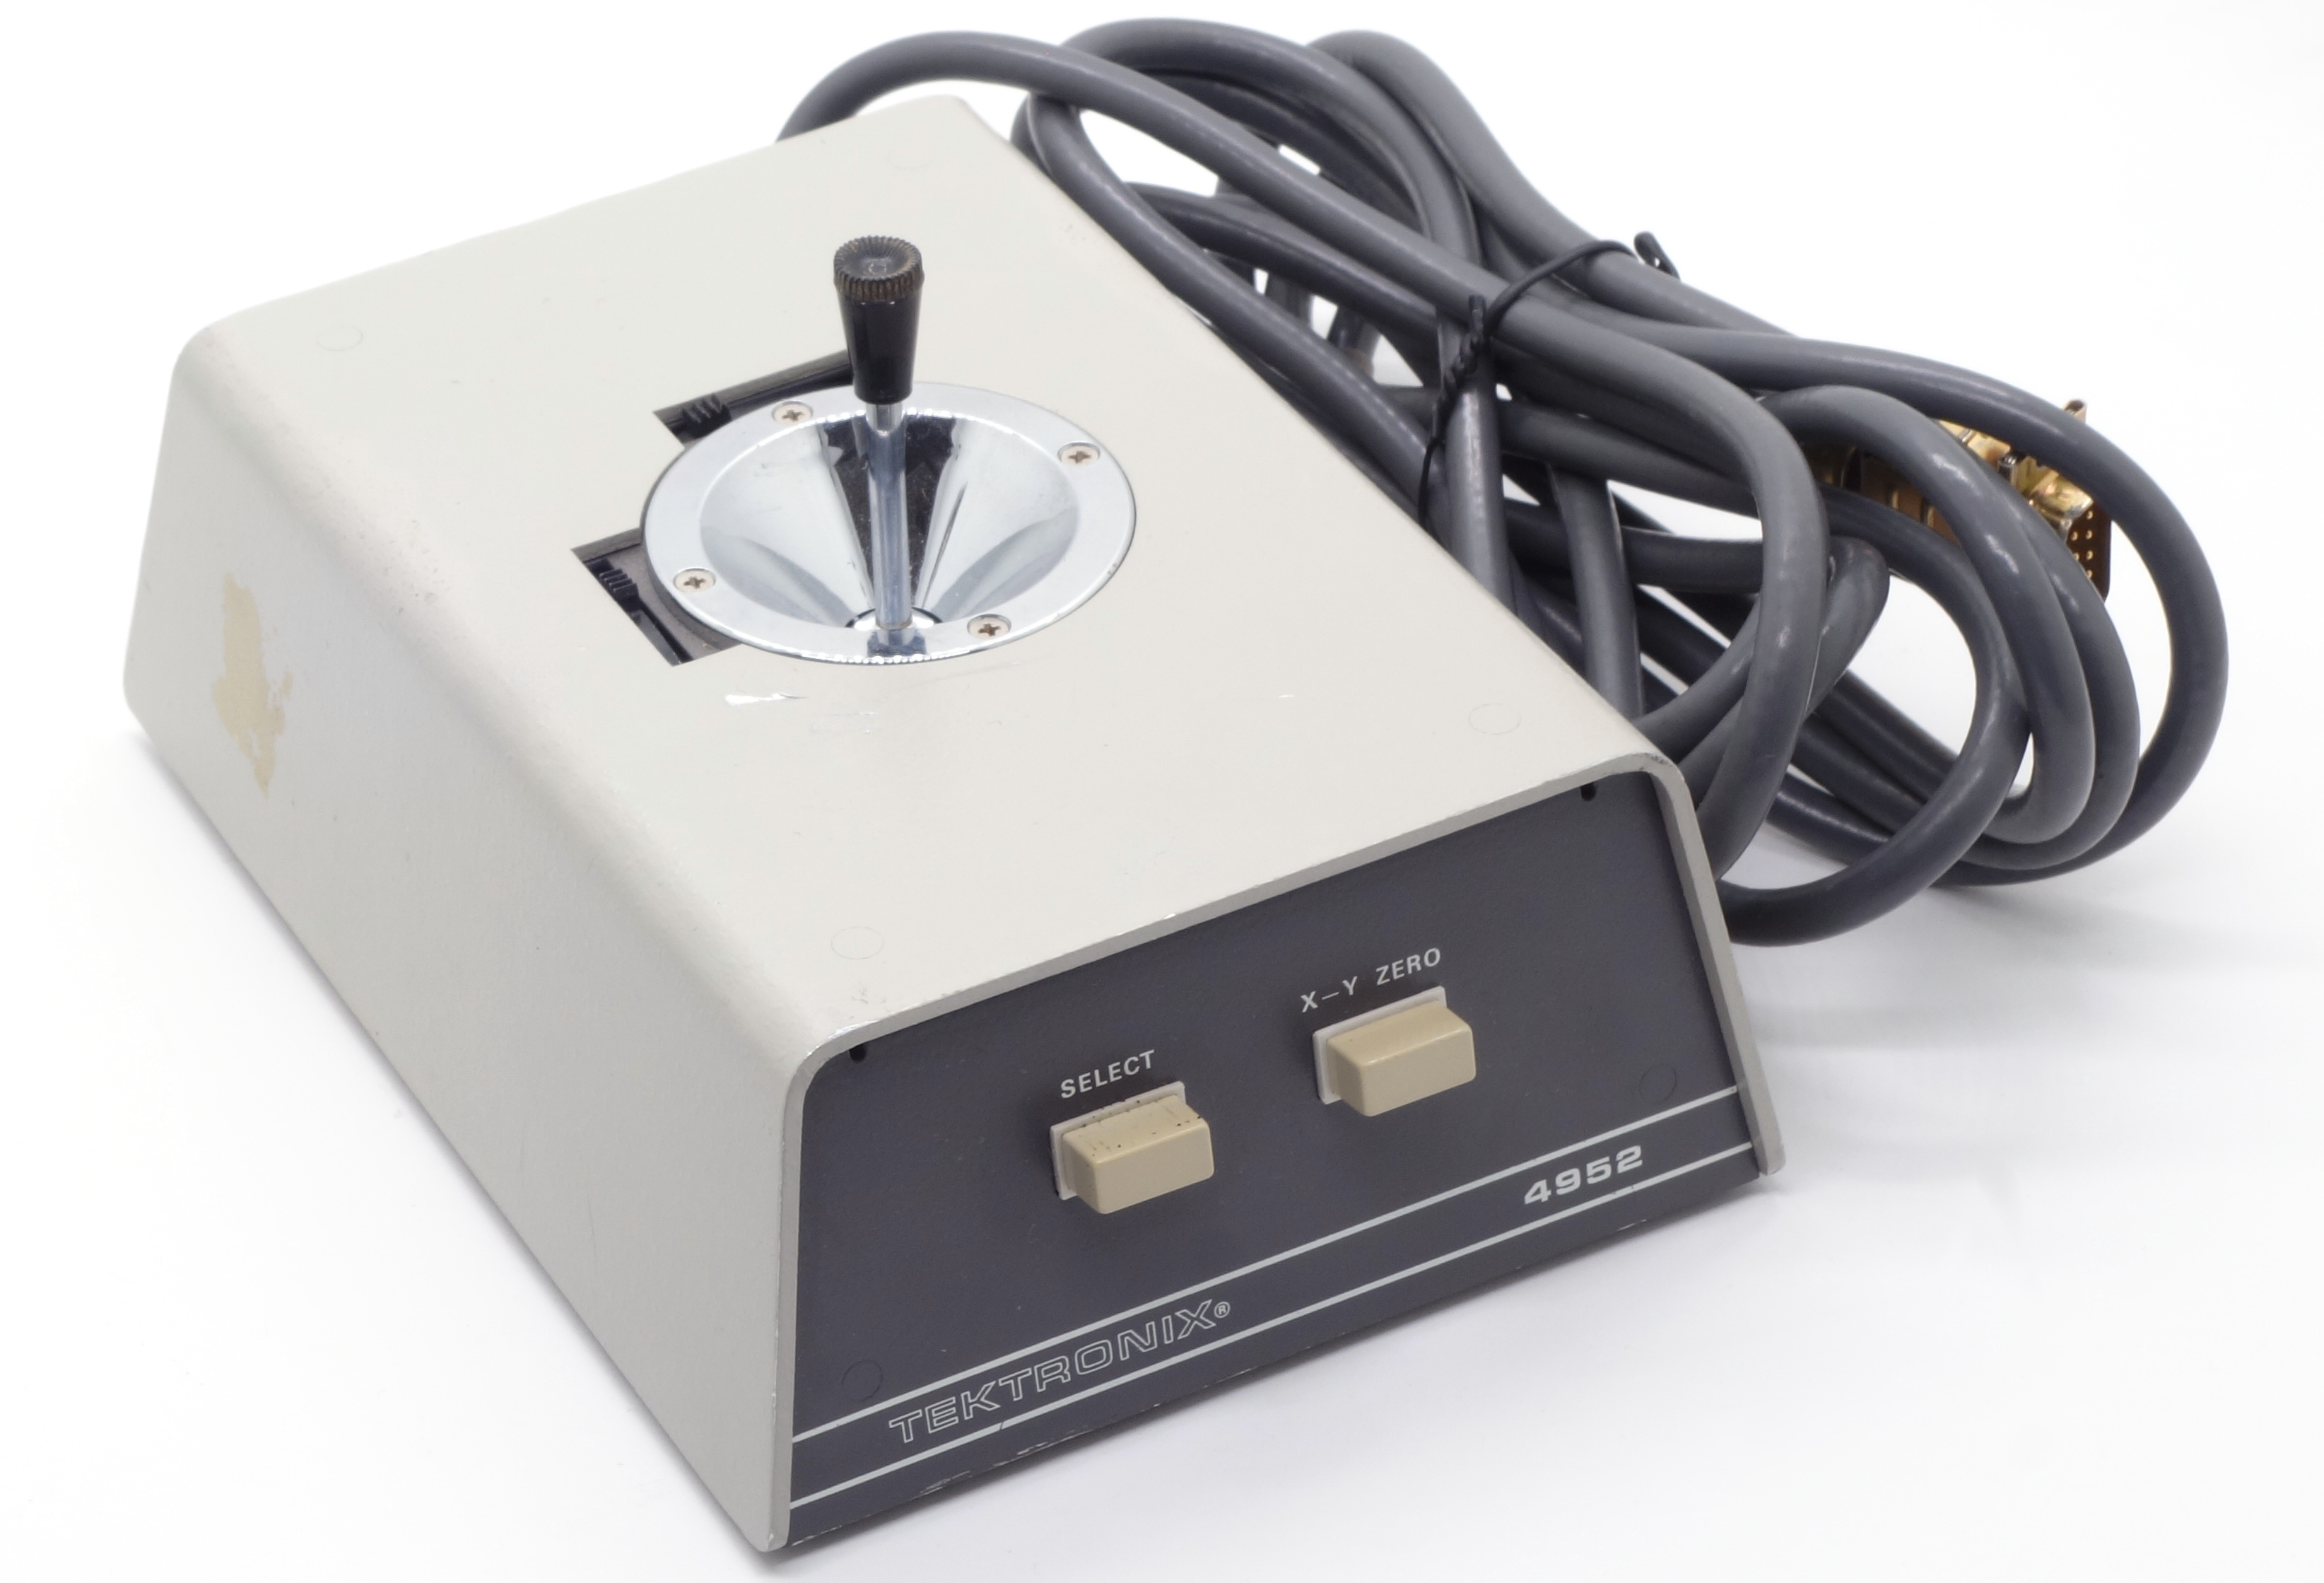
\includegraphics[scale=0.5]{1975_Tektronix_4952_Joystick/pic_30.jpg}
    \caption{Tektronix 4952 joystick}
    \label{fig:TektronixJoystickPic}
\end{figure}

The joystick has four rubber feet and a metal body. Top side (fig. \ref{fig:TektronixJoystickTopAndBottom}) contains two drift trim tabs \cite{manual} near the relatively small ``control lever'' (the stick). The overall look fitted Tektronix terminals and computers which followed all-in-one designs with the display, keyboard, CPU and tape drive in a single desktop case \cite{wiki}.

\begin{figure}[h]
    \centering
    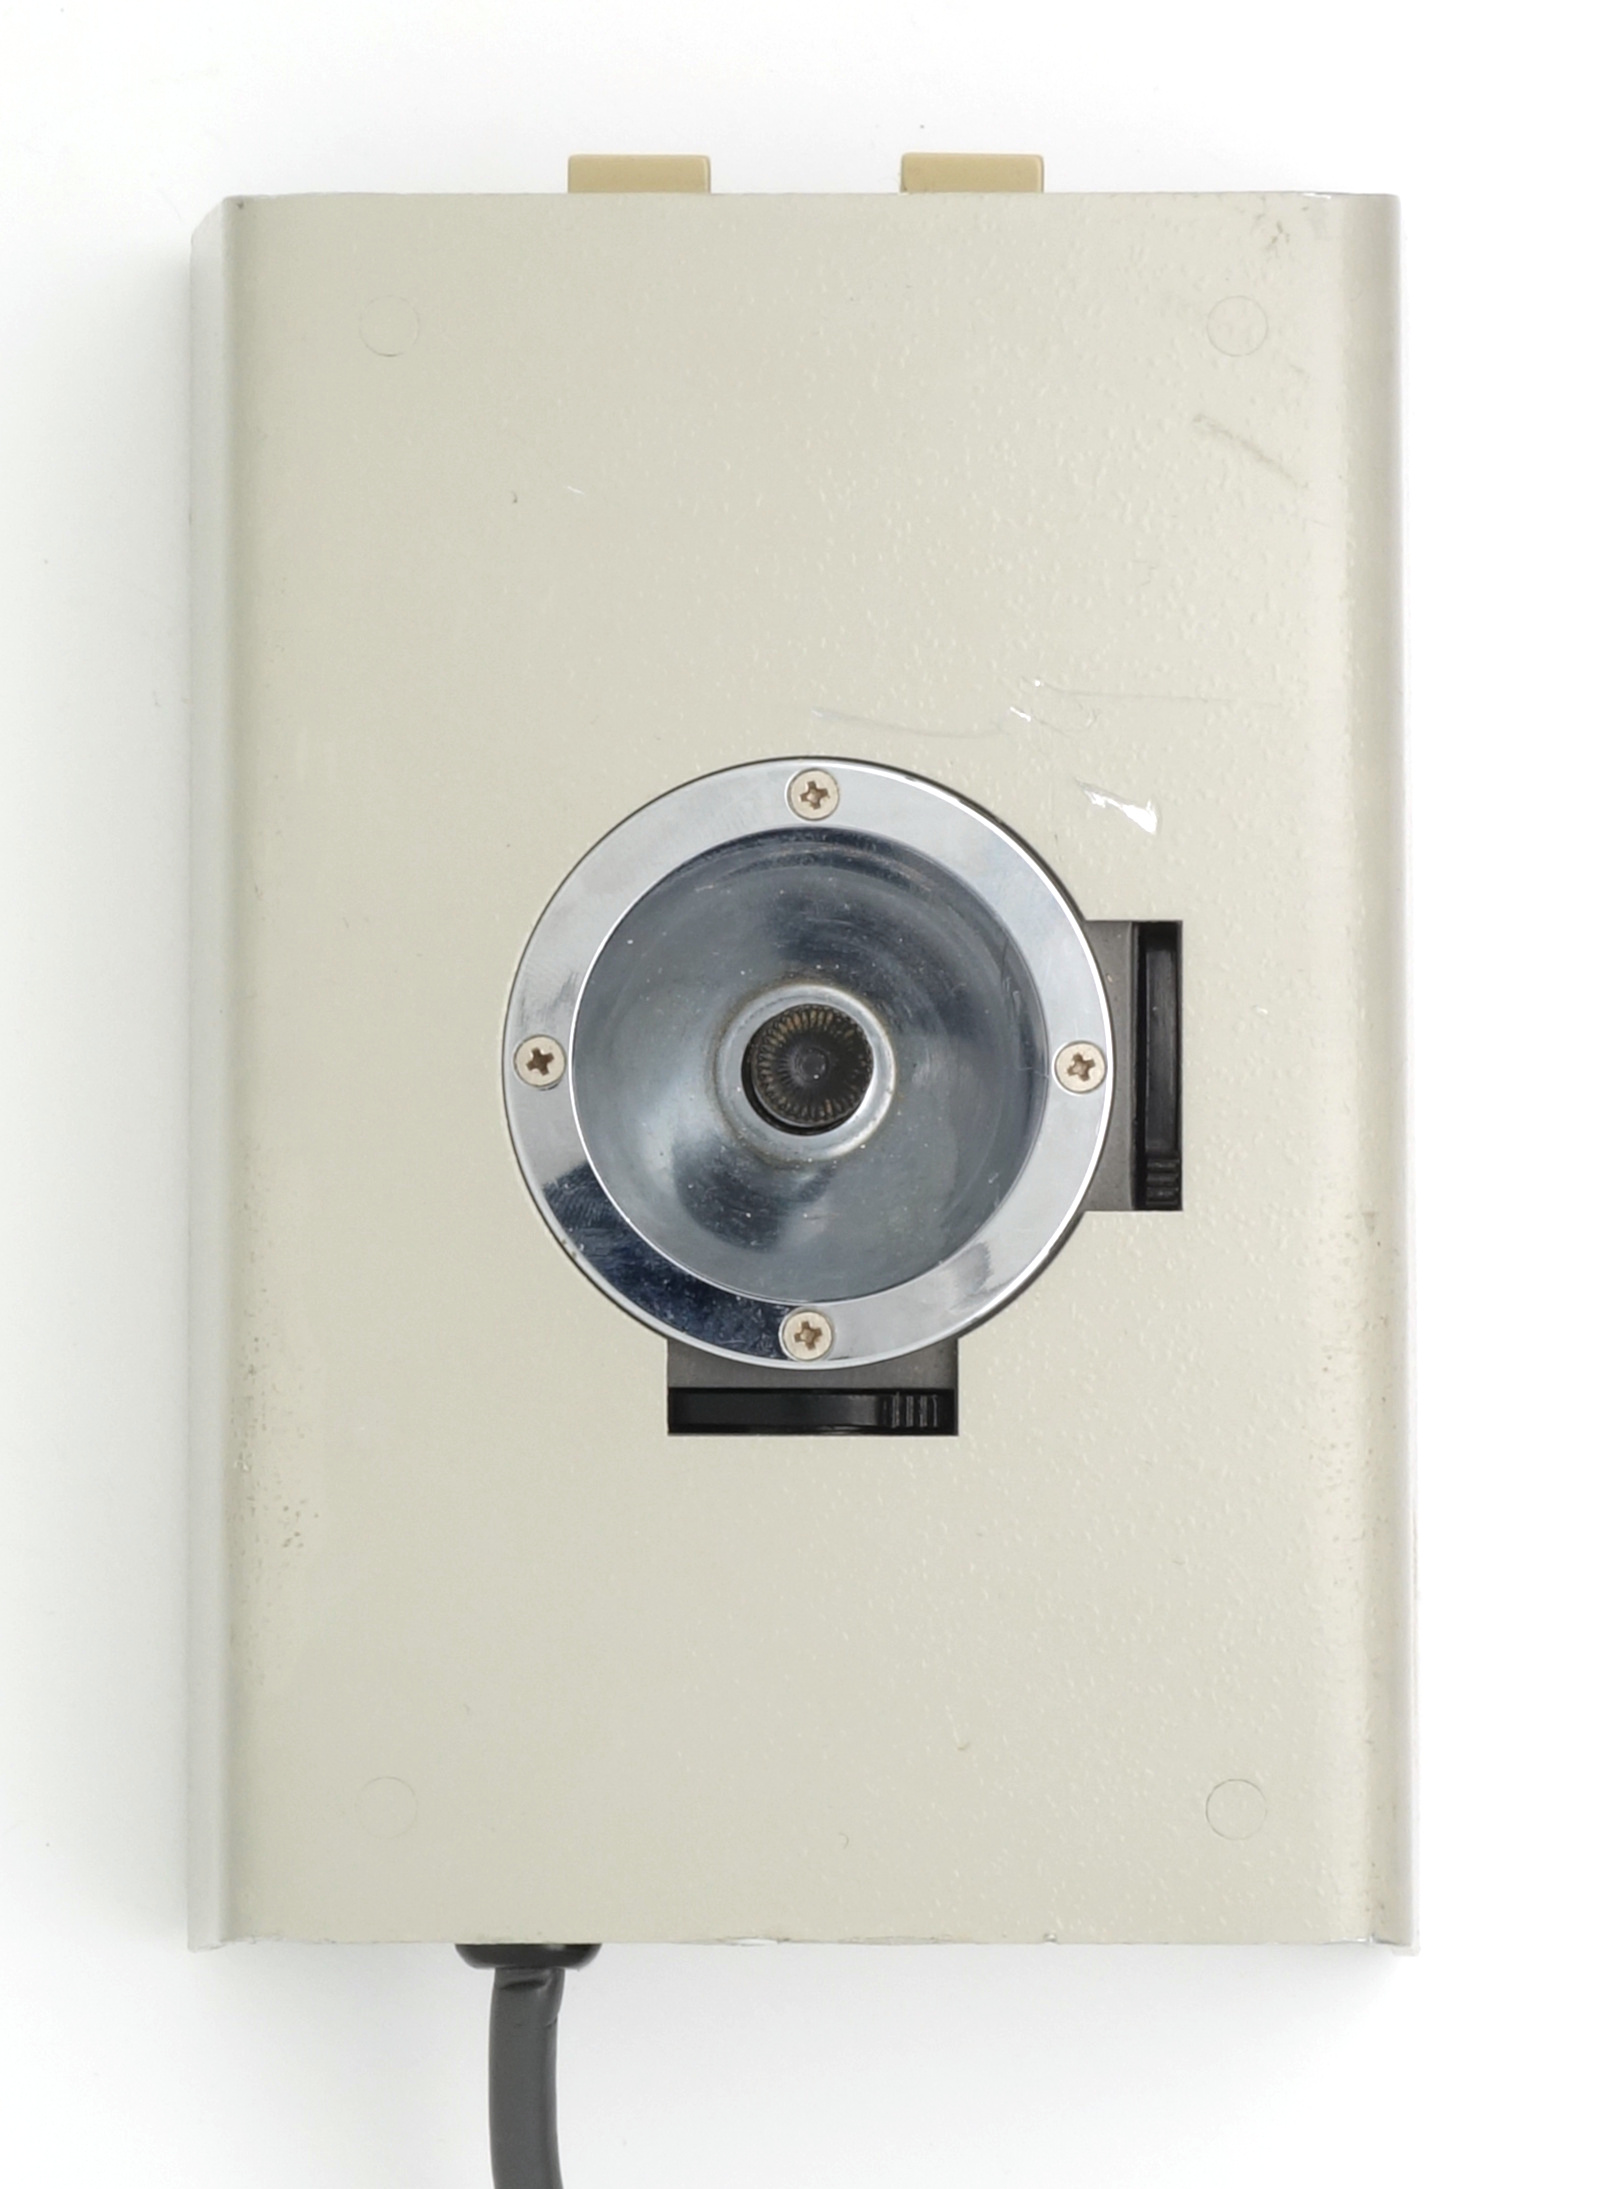
\includegraphics[scale=0.3]{1975_Tektronix_4952_Joystick/top_30.jpg}
    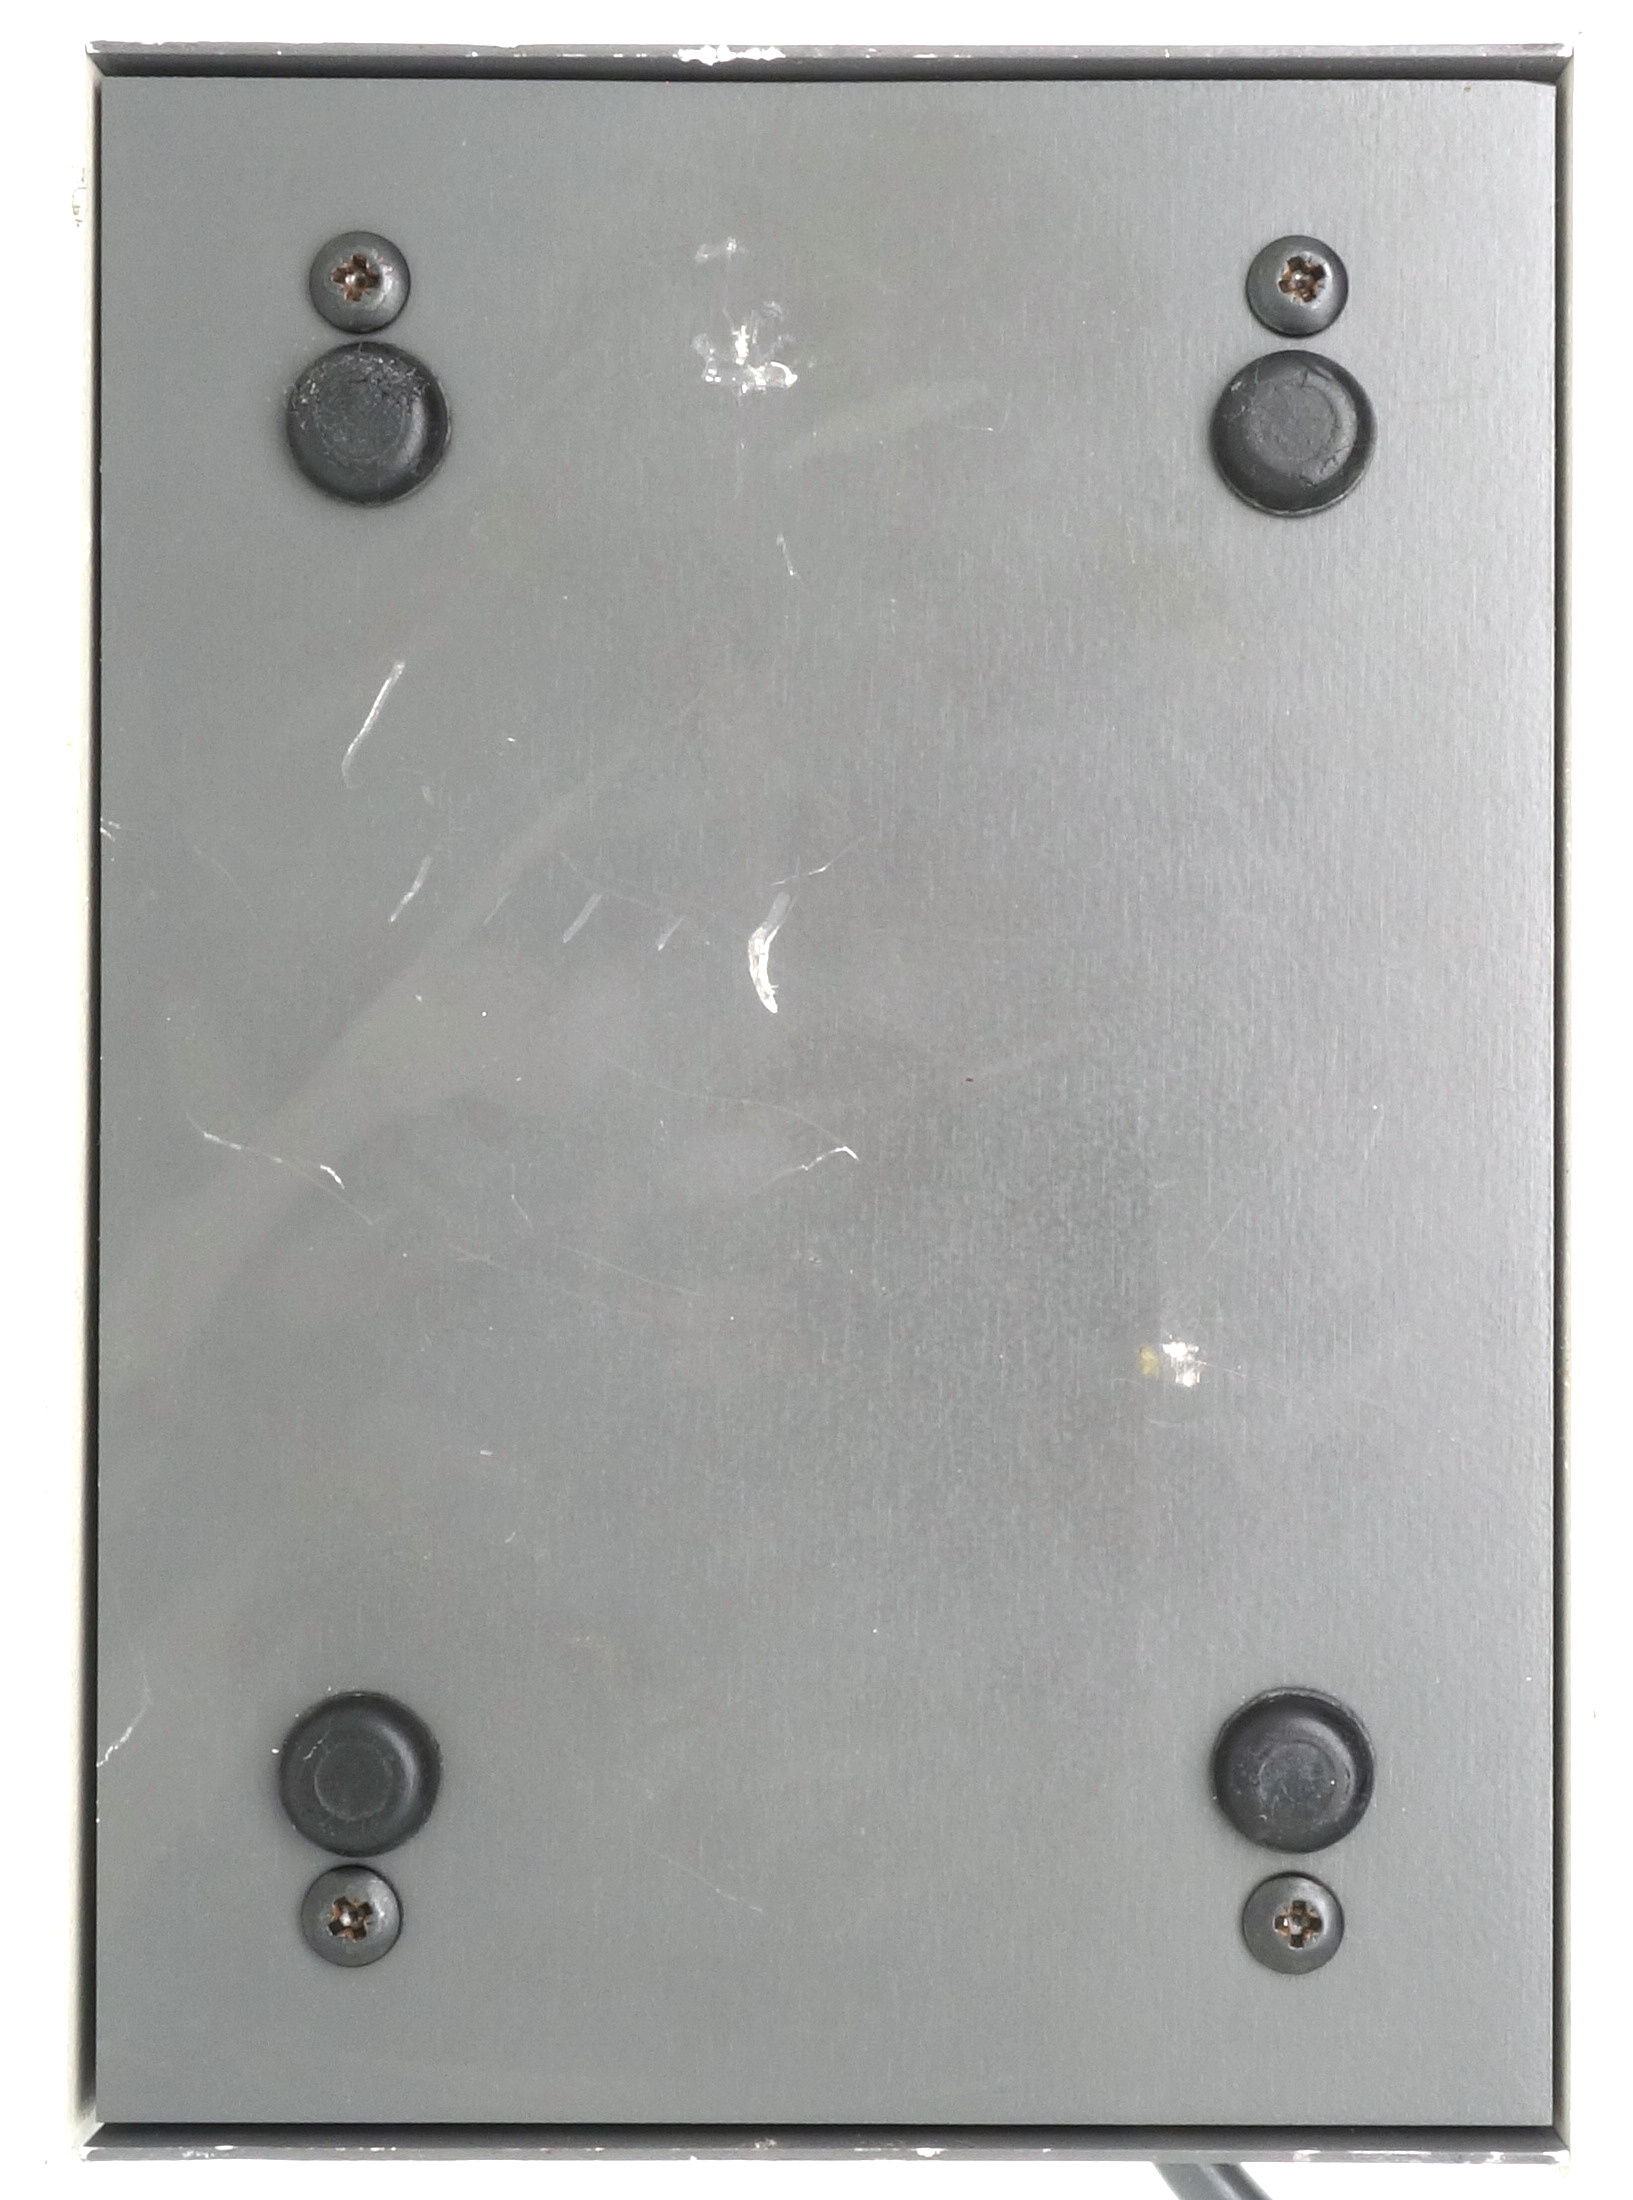
\includegraphics[scale=0.3]{1975_Tektronix_4952_Joystick/bottom_30.jpg}
    \caption{Tektronix 4952 joystick, top and bottom views}
    \label{fig:TektronixJoystickTopAndBottom}
\end{figure}

Front side of the body contains two labeled buttons, Company name and the model of the device.

The body of the unit is really large (fig. \ref{fig:TektronixJoystickSize}).

\begin{figure}[h]
    \centering
    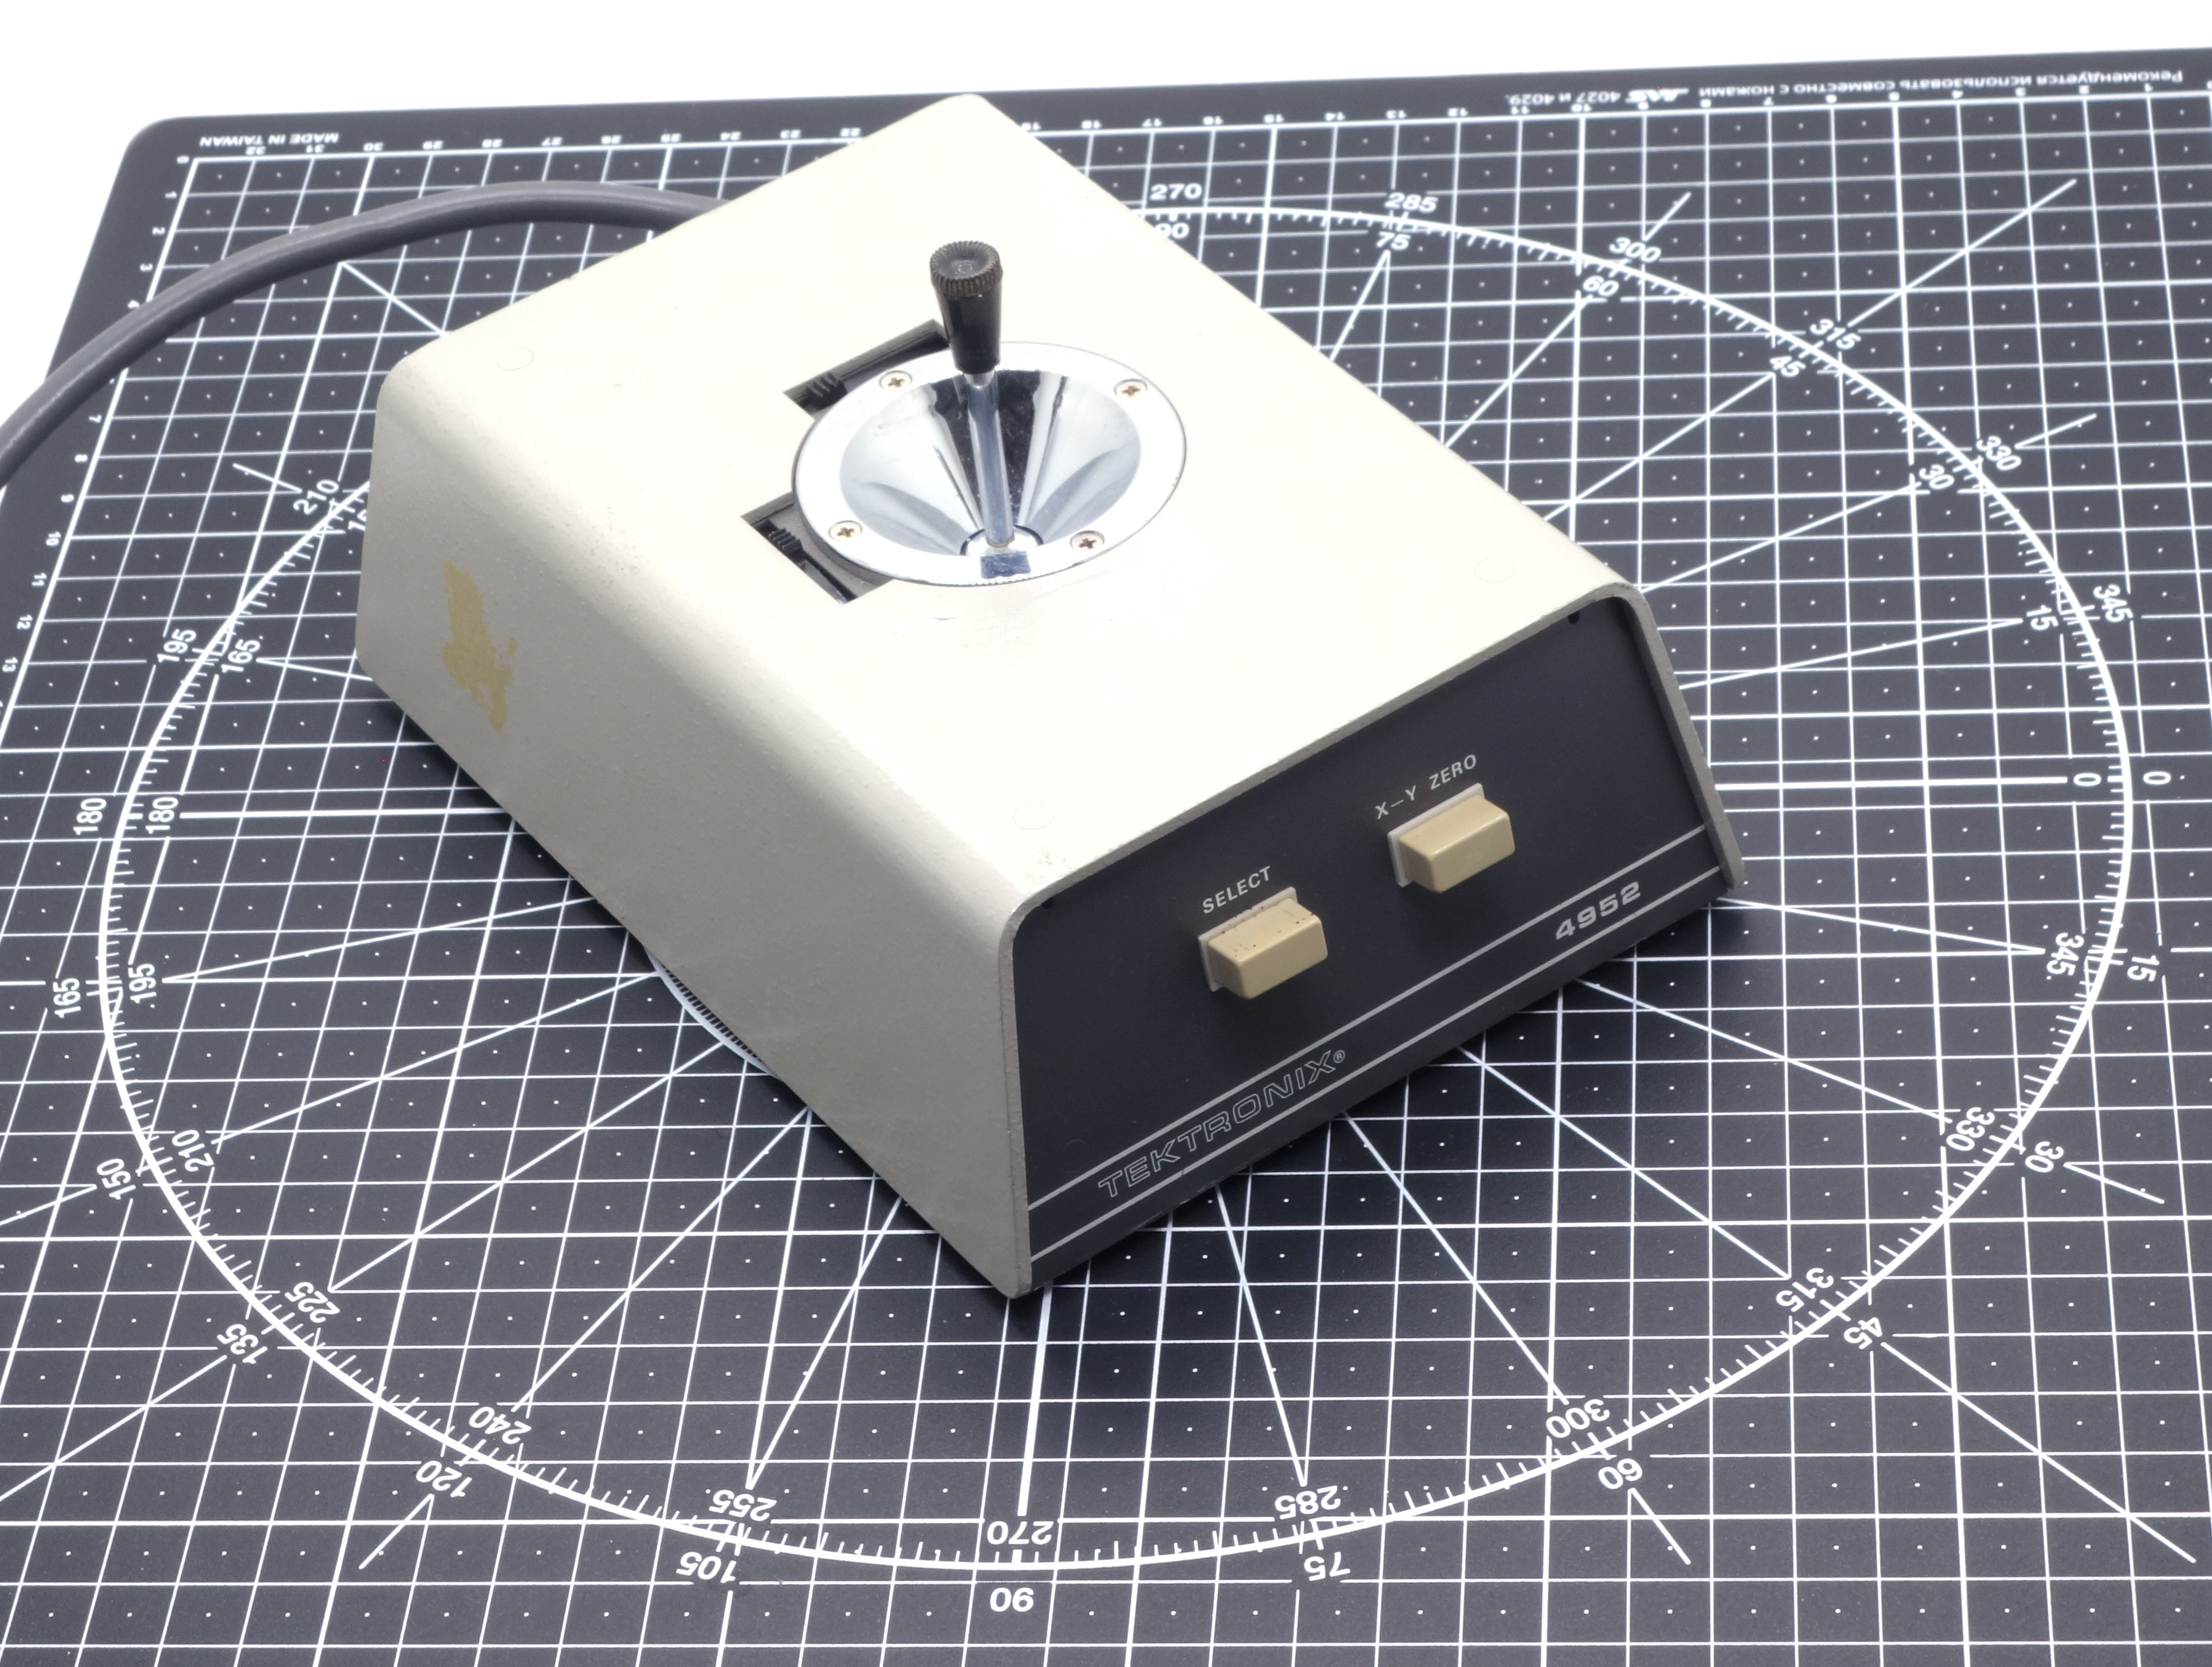
\includegraphics[scale=0.43]{1975_Tektronix_4952_Joystick/size_30.jpg}
    \caption{Tektronix 4952 joystick on a graduated pad with a grid step of 1~cm}
    \label{fig:TektronixJoystickSize}
\end{figure}

It's comfortable enough to move the stick while holding it with fingers and resting your hand on the body, but due to the large size of the body, you cannot reach the buttons on the front panel without removing your hand (fig. \ref{fig:TektronixJoystickHand}). Still, this wasn't a problem because of the usage specifics of the device.

\begin{figure}[h]
    \centering
    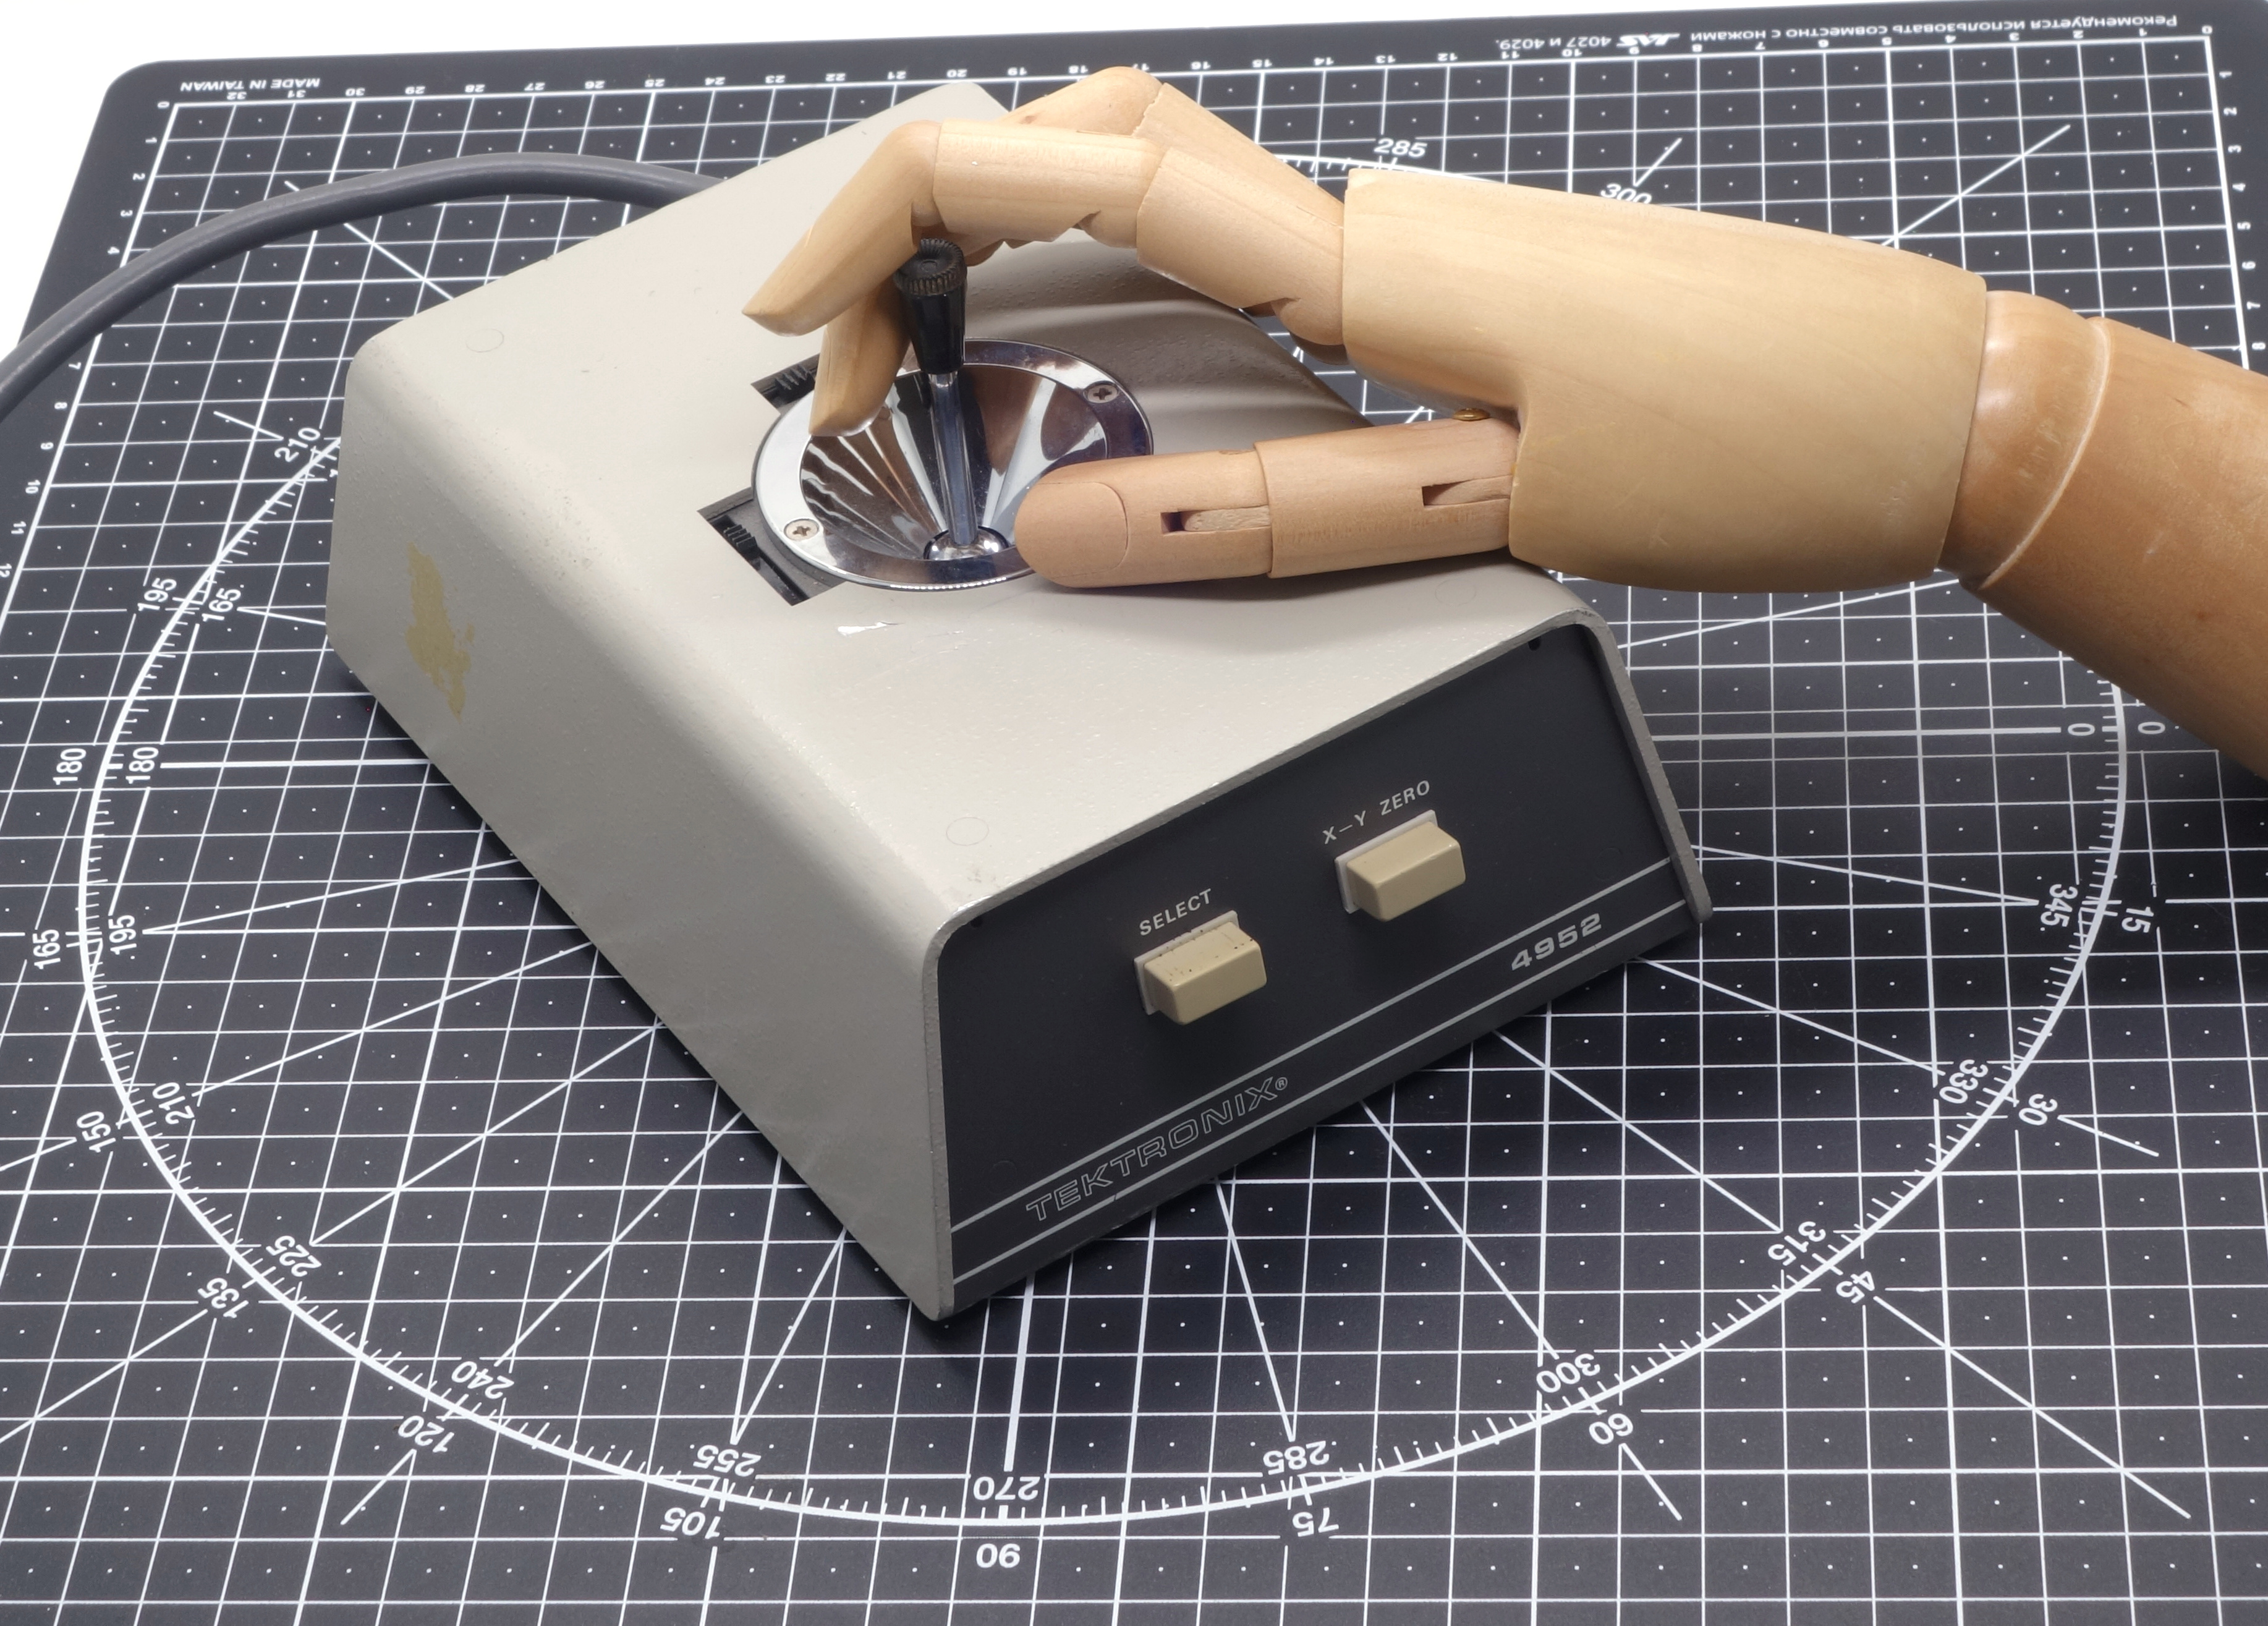
\includegraphics[scale=0.43]{1975_Tektronix_4952_Joystick/hand_05.jpg}
    \caption{Tektronix 4952 joystick with a human hand model}
    \label{fig:TektronixJoystickHand}
\end{figure}

\begin{itemize}
\item \verb!SELECT! is a locking button used only on 4010 graphic terminals: it allowed either the joystick or the thumb-wheels of the terminal to control the ``cross-hair cursor'' position \cite{manual, manual2}. 

\item \verb!X-Y ZERO! push button sets the $X$ and $Y$ outputs of the joystick to zero volts, which immediately moves the cursor to the center of the screen \cite{manual}.
\end{itemize}

Stick tilt affects the cursor movement in a predictable way: direction of the movement is determined by the direction of tilt, while the tilt angle is proportional to the speed of movement. Drift tabs are used to adjust voltage to zero on $X$ and $Y$ outputs when the stick is in its vertical position.

So, the user was supposed to move the cross-hair cursor with the stick until it reaches specific point on a display, and then  cursor coordinates could be obtained by software (for example, some CAD system) when needed \cite{price}.

Joystick was connected to the system using a long thick cable. 4050 series computers included a GPIB parallel bus to connect external peripherals, while 4010 series terminals had special adapter installed into the pedestal of the terminal \cite{manual, manual2}. 

Disassembled joystick is shown in fig. \ref{fig:TektronixJoystickInside}. 

\begin{figure}[h]
    \centering
    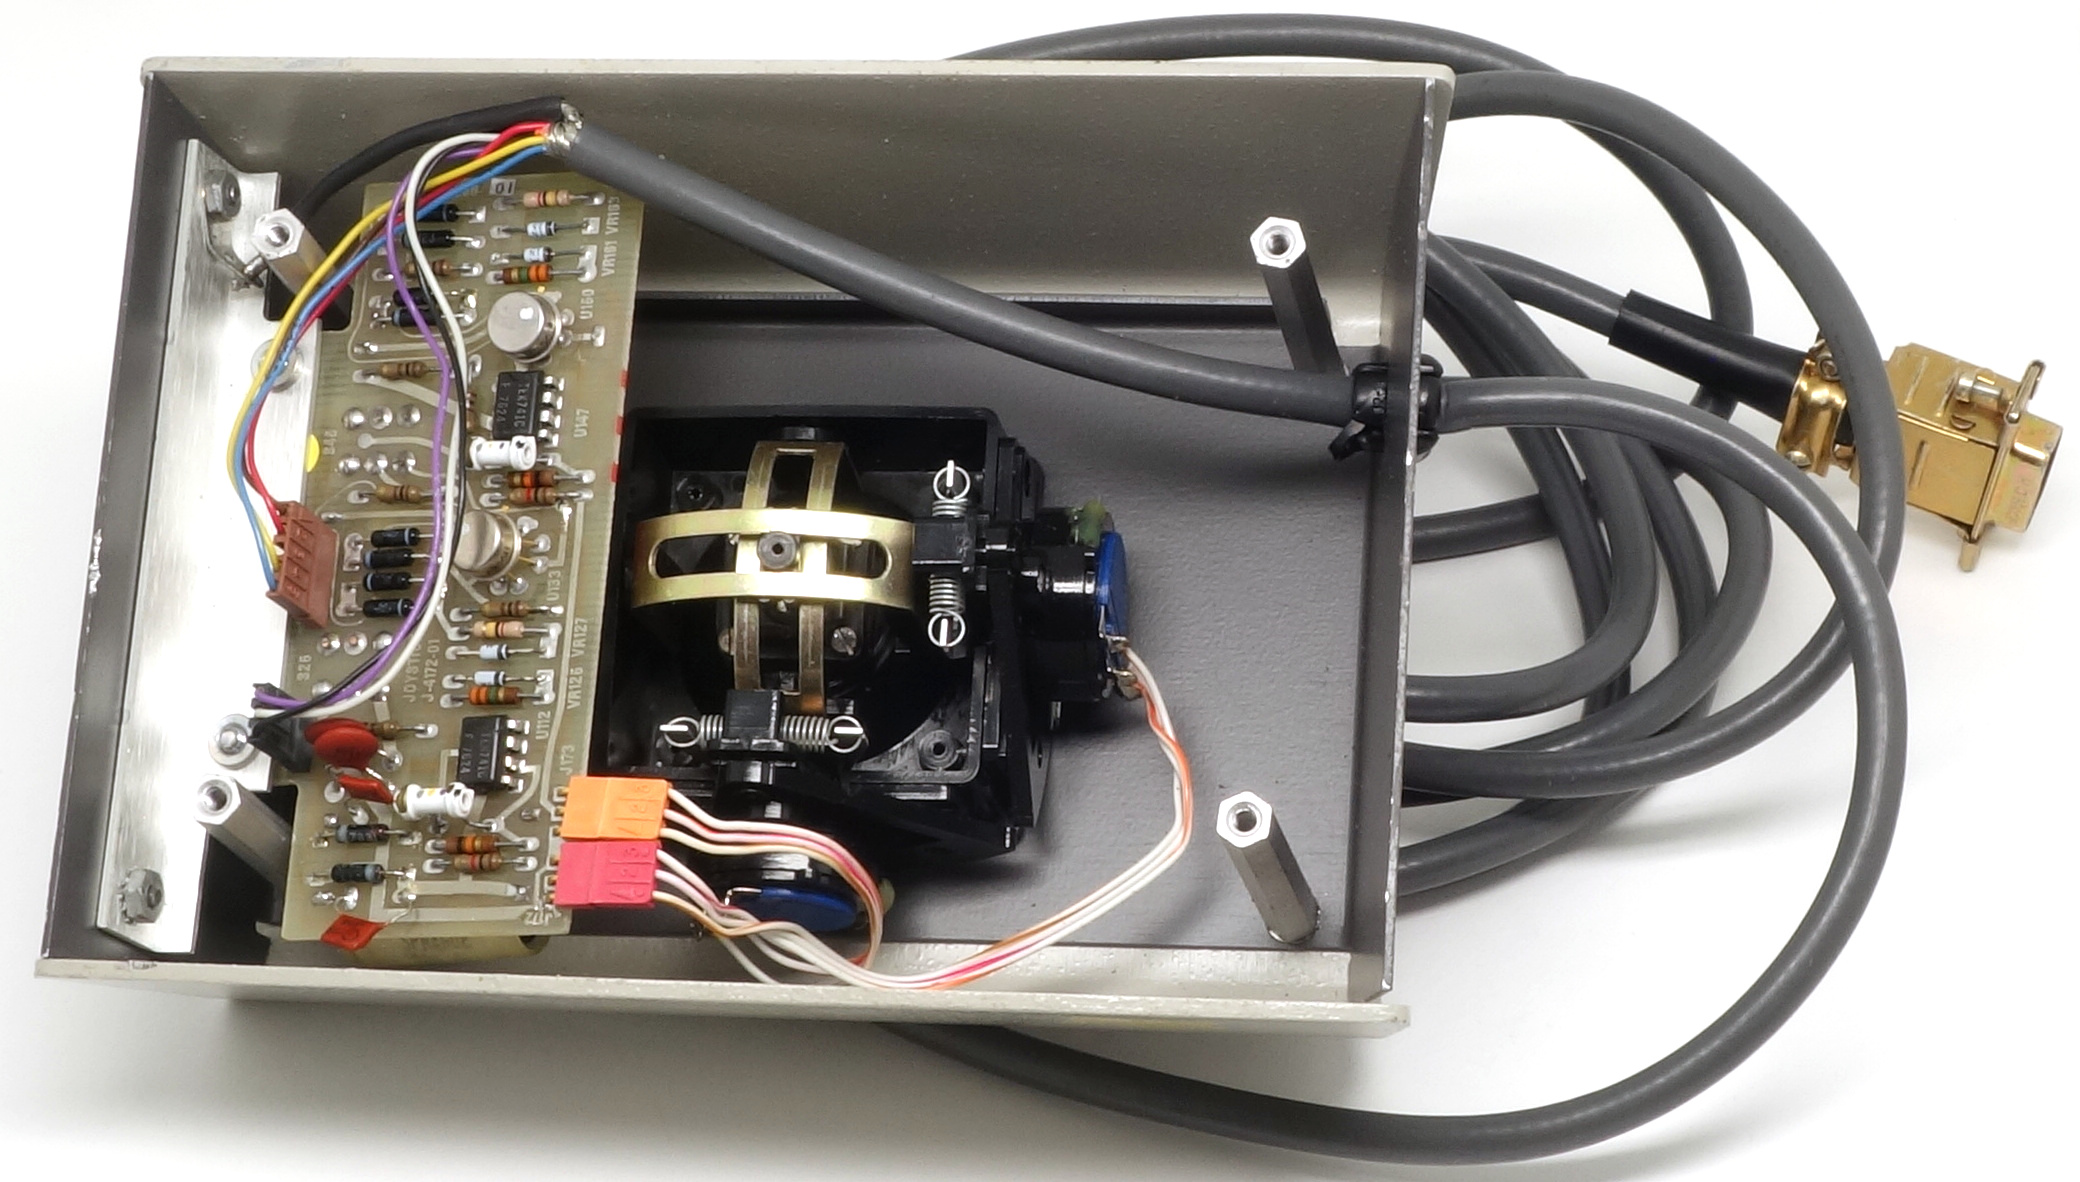
\includegraphics[scale=0.8]{1975_Tektronix_4952_Joystick/inside_30.jpg}
    \caption{Tektronix 4952 joystick disassembled}
    \label{fig:TektronixJoystickInside}
\end{figure}

Trim tabs mechanically rotate the $X$ and $Y$ potentiometers to control drift.
The joystick assembly, including the stick and its mount, as well as potentiometers and coarse drift rotation tabs, is typical: it appears later unchanged up to complete interchangeability in a lot of analog joysticks produced for industrial needs.


\begin{thebibliography}{9}
\bibitem {wiki} Tektronix 4050 -- Wikipedia \url{https://en.wikipedia.org/wiki/Tektronix_4050}
\bibitem {adv} Canadian Information Processing Society (CIPS) Computer Magazine - Vol. 5, Iss. 1-11, 1974. - p. 29
\bibitem {manual} TEKTRONIX 4952 JOYSTICK. Tektronix, Inc., JAN 1975. \url{http://www.bitsavers.org/pdf/tektronix/401x/070-1826-01_4952_Joystick_Jan75.pdf}
\bibitem {manual2} TEKTRONIX 4952 JOYSTICK OPTION 2. Instruction manual Tektronix, Inc., FEB 1976. \url{http://www.bitsavers.org/pdf/tektronix/405x/070-2098-00_4952_Joystick_Feb76.pdf}
\bibitem {price} Stanley J. Tektronix 4952 - Electronixandmore Vintage Electronics and Beyond. -- \url{https://electronixandmore.com/misc/index.php?item=56}
\end{thebibliography}
\end{document}
